\sectionthree{Cantor's Diagonal Trick: Counting $\R$}
\begin{python0}
from solutions import *; clear()
\end{python0}

Instead of showing that $\R$ is bigger than $\N$, I'm going to show 
you that in fact the interval of real numbers 
$[0, 1)$ is already bigger than $\N$.
The proof technique was invented by Georg Cantor, the mathematician
who defined this whole new way of counting by using 1--1 and onto functions.

First of all let me just declare that I'm going to prove our goal by 
contradiction.
I'm going to assume that $[0,1)$ is countable.
Therefore I can list the values in $[0,1)$, say
\[
x_0, x_1, x_2, x_3, \ldots
\]
(The goal
is to show you that I can find a value not in the above list.)

Next, I'm going to express the $x_i$ as decimal numbers.
For instance if $x_0 = 1/2$, then I'm going to write $x_0 = 0.5$ instead.
Furthermore, I'm going to write the numbers with infinitely many decimal
places.
For instance if $x_1 = 0.5$, I'm going to write
\[
x_0 = .5000000000000000\ldots
\]
I'm going to give names to the decimal digits of $x_0$.
The $i$--th digit is written $x_{0i}$
So in this case,
\begin{align*}
x_{00} &= 5 \\
x_{01} &= 0 \\
x_{02} &= 0 \\
x_{03} &= 0 \\
x_{04} &= 0 \\
\end{align*}
etc.
If $x_2$ is $0.14159265...$, then
\begin{align*}
x_{10} &= 1 \\
x_{11} &= 4 \\
x_{12} &= 1 \\
x_{13} &= 5 \\
x_{14} &= 9 \\
\end{align*}
etc.
So far so good ... we have a list of numbers $x_0, x_1, x_2, ...$ 
and a bunch of digits
\begin{align*}
x_{00}, x_{01}, x_{02}, ... \\
x_{10}, x_{11}, x_{12}, ... \\
x_{20}, x_{21}, x_{22}, ... \\
\end{align*}

Let me lay the digits in a grid:

\begin{center}
\begin{tikzpicture}[>=triangle 60,shorten >=0.5pt,node distance=2cm,auto,initial text=, double distance=2pt]
\node[state,initial] (A) at (  0,  0) {$q_0$};
\node[state] (B) at (  4,  0) {$q_1$};
\node[state,accepting] (D) at (  8,  0) {$q_3$};
\node[state] (C) at (  4, -4) {$q_2$};

\path[->]
(A) edge [loop above] node {$a$} ()
(A) edge [bend left=0,pos=0.5,above] node {$\epsilon$} (B)
(A) edge [bend left=0,pos=0.5,above] node {$a$} (C)
(B) edge [bend left=0,pos=0.5,above] node {$b$} (D)
(C) edge [bend left=0,pos=0.5] node {$a,\epsilon$} (B)
(D) edge [bend left=0,pos=0.5] node {$a,b$} (C)

;
\end{tikzpicture}
\end{center}
    

I will fill the cell at row $x_i$ and column $j$ with the $x_{ij}$.
For instance since $x_0 = 0.5000\ldots$ and $x_1 = 0.14159254\ldots$,
I have the following:
\begin{center}
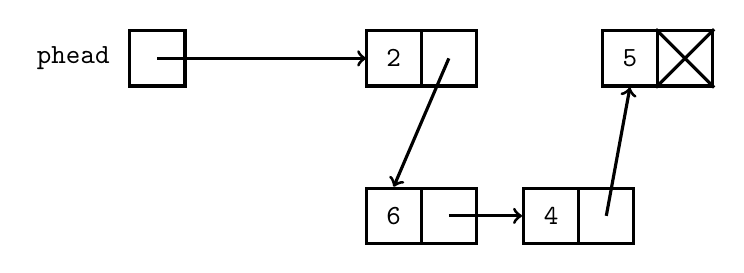
\begin{tikzpicture}

\draw (0.35, 0.35)
  node[draw, line width=0.04cm, , color=black,
       rounded corners=0cm, inner sep=0cm] {

\begin{minipage}[t][0.7cm]{0.7cm}
\mbox{}

\end{minipage}

};\draw (0.35, 0.35) node[color=black] {{\texttt{2}}};
\draw (1.0499999999999998, 0.35)
  node[draw, line width=0.04cm, , color=black,
       rounded corners=0cm, inner sep=0cm] {

\begin{minipage}[t][0.7cm]{0.7cm}
\mbox{}

\end{minipage}

};\draw (1.0499999999999998, 0.35) node[color=black] {{\texttt{}}};
\draw (0.35, -1.65)
  node[draw, line width=0.04cm, , color=black,
       rounded corners=0cm, inner sep=0cm] {

\begin{minipage}[t][0.7cm]{0.7cm}
\mbox{}

\end{minipage}

};\draw (0.35, -1.65) node[color=black] {{\texttt{6}}};
\draw (1.0499999999999998, -1.65)
  node[draw, line width=0.04cm, , color=black,
       rounded corners=0cm, inner sep=0cm] {

\begin{minipage}[t][0.7cm]{0.7cm}
\mbox{}

\end{minipage}

};\draw (1.0499999999999998, -1.65) node[color=black] {{\texttt{}}};
\draw (2.35, -1.65)
  node[draw, line width=0.04cm, , color=black,
       rounded corners=0cm, inner sep=0cm] {

\begin{minipage}[t][0.7cm]{0.7cm}
\mbox{}

\end{minipage}

};\draw (2.35, -1.65) node[color=black] {{\texttt{4}}};
\draw (3.0500000000000003, -1.65)
  node[draw, line width=0.04cm, , color=black,
       rounded corners=0cm, inner sep=0cm] {

\begin{minipage}[t][0.7cm]{0.7cm}
\mbox{}

\end{minipage}

};\draw (3.0500000000000003, -1.65) node[color=black] {{\texttt{}}};
\draw (3.35, 0.35)
  node[draw, line width=0.04cm, , color=black,
       rounded corners=0cm, inner sep=0cm] {

\begin{minipage}[t][0.7cm]{0.7cm}
\mbox{}

\end{minipage}

};\draw (3.35, 0.35) node[color=black] {{\texttt{5}}};
\draw (4.05, 0.35)
  node[draw, line width=0.04cm, , color=black,
       rounded corners=0cm, inner sep=0cm] {

\begin{minipage}[t][0.7cm]{0.7cm}
\mbox{}

\end{minipage}

};\draw (4.05, 0.35) node[color=black] {{\texttt{}}};\draw[line width=0.04cm,black,->] (1.05,0.35) to  (0.35,-1.28);
\draw[line width=0.04cm,black,->] (1.05,-1.65) to  (1.98,-1.65);
\draw[line width=0.04cm,black,->] (3.05,-1.65) to  (3.35,-0.02);
\draw[line width=0.04cm,black] (3.68,0.72) to  (4.42,-0.02);
\draw[line width=0.04cm,black] (4.42,0.72) to  (3.68,-0.02);

\draw (-2.65, 0.35)
  node[draw, line width=0.04cm, , color=black,
       rounded corners=0cm, inner sep=0cm] {

\begin{minipage}[t][0.7cm]{0.7cm}
\mbox{}

\end{minipage}

};\draw (-2.65, 0.35) node[color=black] {{\texttt{}}};\draw[line width=0.04cm,black,->] (-2.65,0.35) to  (0,0.35);

\draw (-3.7199999999999998, 0.35)
  node[draw, line width=0.04cm, , color=white,
       rounded corners=0cm, inner sep=0cm] {

\begin{minipage}[t][0.1cm]{0.1cm}
\mbox{}

\end{minipage}

};\draw (-3.7199999999999998, 0.35) node[color=black] {{\texttt{phead}}};
\end{tikzpicture}

\end{center}



Now I'm going to construct a value $y$ that is in $[0,1)$ that is
not in the above list.
I'm going to build $y$ by specifying the decimals of $y$.
Just like the $x_i$'s above, $y$ is going to look like this:
\[
y = 0.y_0 y_1 y_2 \cdots
\]
where $y_i$ is the $i$--digit of $y$ to the right of the decimal point.
In order for $y$ to contradict our assumption about 
the countability of $[0,1)$,
I will need $y$ not to be $x_0$, and not be $x_1$, and not be $x_2$, etc.

To make $y$ not $x_0$, I look at the first digit of $x_0$ to the right
of the decimal place, i.e., $x_{00}$.
All I need to do is to choose $y_0$ to be different from $x_{00}$.
For instance if $x_{00} = 5$, 
I can choose $0$ for $y_0$ (of course I can also choose $1$
for $y_0$ ... any digit that is not 5 works.)
In other words I make $y$ \textit{not} $x_0$ by making them different
at the first decimal place.

So at this point $y$ looks like
\[
y = 0.0y_2 y_3 \cdots
\]

Now suppose the second digit of $x_1$ to the right of the decimal point
is $1$.
Using the same trick, I will choose $y_1$ to be different from $x_{11} = 1$.
For instance I can choose $y_1 = 7$.
At this point
\[
y = 0.07 y_3 y_4 y_5 \cdots
\]

Etc.

In general, for $i \geq 0$, $y_{ii}$ to be an element in
\[
\{0, 1, 2, \ldots, 9\} - \{x_{ii}\}
\]
This will ensure that
\[
y \neq x_i
\]

Note that the form of $y$ tells me that $y$ is indeed in $[0,1)$.
We have found a value, $y$, in $[0,1)$ which is not in the list
\[
x_1, x_2, x_3, ...
\] 
which I assumed at the beginning is a complete list of values in $[0,1)$.

Contradiction!!!

Actually there's a small point:
What if I accidentally select $y_0 = 9$, $y_1 = 9$, $y_2 = 9$, ...
This means that $y$ looks like $0.9999\cdots$.
This value is not in $[0,1)$.
This value is actually $1$ and it not in $[0,1)$.
(Right? Check with your math textbooks or with your math instructors.)
In the same way $0.499999\cdots$ is actually the same as
$0.5$.
To avoid issues like these, I will just make sure that I will never choose
$9$ for the $y_i$'s.
Problem fixed!!!

This proof technique is called the \defone{Cantor's diagonal trick}
(or Cantor's diagonal method if you want to make it sound more respectable.)

\begin{thm}
$\R$ is not countable.
\end{thm}

Now you might think that $[0,1)$ is much smaller than $\R$.
But in fact ...

%-*-latex-*-

\begin{ex} 
  \label{ex:prob-00}
  \tinysidebar{\debug{exercises/{disc-prob-28/question.tex}}}

  \solutionlink{sol:prob-00}
  \qed
\end{ex} 
\begin{python0}
from solutions import *
add(label="ex:prob-00",
    srcfilename='exercises/discrete-probability/prob-00/answer.tex') 
\end{python0}


\newpage
I am now going to show you that there is a language
(over a fixed $\Sigma$ throughout this argument of course, 
say $\Sigma = \{a,b\}$)
which is not accepted by a Turing machine, i.e.,
the language is not Turing--recognization (or recursively enumerable.)

I'll do this in two different ways:
the first way is to show that there
are more languages than Turing machines (the method is by counting)
and the second way is by defining a language that is not Turing--recognizable.

First of all ... how many Turing machines are there?
The number of Turing machines is actually countable.

Why?

Because each Turing machine can be encoded as a finite binary string.
This means that the collection of Turing machines
is a subset of 
\[
\Sigma^* 
= \bigcup_{n=0}^\infty \Sigma^n 
= \Sigma^0 \cup \Sigma^1 \cup \Sigma^2 \cup \cdots
\]
Note that each of the $\Sigma^n$ is countable (in fact finite!)
Therefore $\Sigma^*$ is a countable union of countable sets.
This implies that $\Sigma^*$ is countable.

\begin{thm}
The set of Turing machines (for a fixed $\Sigma$) is countable.
\end{thm}

Before we count $\LANG_\Sigma$,
the collection of languages of $\Sigma$,
let's try another counting example that involves Cantor's diagonal trick.

Let's count the number of functions from $\N$ to $\{0, 1\}$.
An element of this set is of the from
\[
f: \N \rightarrow \{0, 1\}
\]
For convenience, let me call this set $X$.
I claim that $X$ is not countable.
By my assumption, I can list the elements in $X$ like this:
\[
f_0, f_1, f_2, \ldots
\]
$f_0$ is of course completely determined by 
\[
f_0(0), f_0(1), f_0(2), f_0(3), \ldots
\]
Each $f_i(j)$ is either 0 or 1.
Now I'm going to build a function $g : \N \rightarrow \{0, 1\}$
which is not in the above list.
How?

This is actually very similar to the setup in Cantor's argument
above.
In this case we have:

\begin{center}
\begin{tikzpicture}
\draw[line width=0.03cm,red,<->] (7) to [bend left=90]  (8);

\fill[blue!10] (0.0, 0.0) circle (0.35);
\node [line width=0.03cm,black,minimum size=0.6699999999999999cm,draw,circle] at (0.0,0.0)(10){};\draw (0.0, 0.0) node[color=black] {\texttt{10}};
\fill[blue!10] (-0.95, -1.0) circle (0.35);
\node [line width=0.03cm,black,minimum size=0.6699999999999999cm,draw,circle] at (-0.95,-1.0)(5){};\draw (-0.95, -1.0) node[color=black] {\texttt{5}};
\fill[blue!10] (0.95, -1.0) circle (0.35);
\node [line width=0.03cm,black,minimum size=0.6699999999999999cm,draw,circle] at (0.95,-1.0)(7){};\draw (0.95, -1.0) node[color=black] {\texttt{7}};
\fill[blue!10] (-1.43, -2.0) circle (0.35);
\node [line width=0.03cm,black,minimum size=0.6699999999999999cm,draw,circle] at (-1.43,-2.0)(2){};\draw (-1.43, -2.0) node[color=black] {\texttt{2}};
\fill[blue!10] (-0.47, -2.0) circle (0.35);
\node [line width=0.03cm,black,minimum size=0.6699999999999999cm,draw,circle] at (-0.47,-2.0)(1){};\draw (-0.47, -2.0) node[color=black] {\texttt{1}};
\fill[blue!10] (0.47, -2.0) circle (0.35);
\node [line width=0.03cm,black,minimum size=0.6699999999999999cm,draw,circle] at (0.47,-2.0)(0){};\draw (0.47, -2.0) node[color=black] {\texttt{0}};
\fill[blue!10] (1.43, -2.0) circle (0.35);
\node [line width=0.03cm,black,minimum size=0.6699999999999999cm,draw,circle] at (1.43,-2.0)(8){};\draw (1.43, -2.0) node[color=black] {\texttt{8}};\draw[line width=0.03cm,black] (10) to  (5);
\draw[line width=0.03cm,black] (10) to  (7);
\draw[line width=0.03cm,black] (5) to  (2);
\draw[line width=0.03cm,black] (5) to  (1);
\draw[line width=0.03cm,black] (7) to  (0);
\draw[line width=0.03cm,black] (7) to  (8);
\end{tikzpicture}

\end{center}



where the cell at row $f_i$ and column $j$ is filled with the
value of $f_i(j)$.
For instance if the table looks like this:
\begin{center}
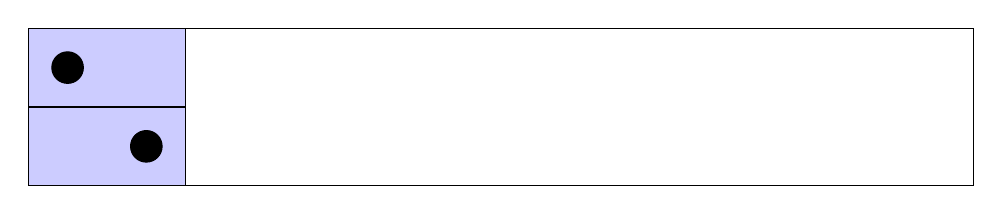
\begin{tikzpicture}

\draw (6.0, 1.0)
  node[draw, , , color=black,
       rounded corners=0cm, inner sep=0cm] {

\begin{minipage}[t][2cm]{12cm}
\mbox{}

\end{minipage}

};
\draw (1.0, 1.5)
  node[fill=blue!20!white,rounded corners=0cm,inner sep=0cm] {

\begin{minipage}[t][1cm]{2cm}
\mbox{}

\end{minipage}

};
\draw (1.0, 1.5)
  node[draw, , , color=black,
       rounded corners=0cm, inner sep=0cm] {

\begin{minipage}[t][1cm]{2cm}
\mbox{}

\end{minipage}

};
\fill[black] (0.5, 1.5) circle (0.2);
\draw[black] (0.5, 1.5) circle (0.2);
\draw (1.0, 0.5)
  node[fill=blue!20!white,rounded corners=0cm,inner sep=0cm] {

\begin{minipage}[t][1cm]{2cm}
\mbox{}

\end{minipage}

};
\draw (1.0, 0.5)
  node[draw, , , color=black,
       rounded corners=0cm, inner sep=0cm] {

\begin{minipage}[t][1cm]{2cm}
\mbox{}

\end{minipage}

};
\fill[black] (1.5, 0.5) circle (0.2);
\draw[black] (1.5, 0.5) circle (0.2);
\end{tikzpicture}

\end{center}



Then $f_0(0) = 1$ and $f_1(2) = 0$, etc.

Well, $g$ is completely determined by 
\[
g(0), g(1), g(2), g(3), ...
\]
So I need to specify $g(n)$ for $n \geq 0$.
For $g(0)$, I'm going to choose a value for $g(0)$ so that 
$g$ is not $f_0$.
Well, that's easy ... I follow Cantor's diagonal trick
and choose $g(0)$ to be different from $f_0(0)$.
If $f_0(0)$ is $1$, I will set $g(0) = 0$.
If $f_0(1)$ is $0$, I will set $g(0) = 1$.
Likewise, I choose a value for $g(1)$ so that $g(1) \neq f_1(1)$.
Etc.

In general I construct my function $g$ such that
for each $n \geq 0$,
\[
g(n)
= 
\begin{cases}
0 & \text{ if } f_n(n) = 1 \\
1 & \text{ if } f_n(n) = 0 \\
\end{cases}
\]
I have constructed a function $g : \N \rightarrow \{0, 1\}$
such that $g \neq f_0$, $g \neq f_1$, ...
Therefore the list of functions $f_0, f_1, f_2, \ldots$ cannot be 
complete.

Therefore $X$ is not countable.
Let's put it down as a theorem ...

\begin{thm}
The set of functions from $\N$ to $\{0,1\}$ is not countable.
\end{thm}

%-*-latex-*-

\begin{ex} 
  \label{ex:prob-00}
  \tinysidebar{\debug{exercises/{disc-prob-28/question.tex}}}

  \solutionlink{sol:prob-00}
  \qed
\end{ex} 
\begin{python0}
from solutions import *
add(label="ex:prob-00",
    srcfilename='exercises/discrete-probability/prob-00/answer.tex') 
\end{python0}


%-*-latex-*-

\begin{ex} 
  \label{ex:prob-00}
  \tinysidebar{\debug{exercises/{disc-prob-28/question.tex}}}

  \solutionlink{sol:prob-00}
  \qed
\end{ex} 
\begin{python0}
from solutions import *
add(label="ex:prob-00",
    srcfilename='exercises/discrete-probability/prob-00/answer.tex') 
\end{python0}


%-*-latex-*-

\begin{ex} 
  \label{ex:prob-00}
  \tinysidebar{\debug{exercises/{disc-prob-28/question.tex}}}

  \solutionlink{sol:prob-00}
  \qed
\end{ex} 
\begin{python0}
from solutions import *
add(label="ex:prob-00",
    srcfilename='exercises/discrete-probability/prob-00/answer.tex') 
\end{python0}

